\documentclass{article}
\usepackage
[
        a4paper,% other options: a3paper, a5paper, etc
        left=2cm,
        right=2cm,
        top=2cm,
        bottom=2cm,
        % use vmargin=2cm to make vertical margins equal to 2cm.
        % us  hmargin=3cm to make horizontal margins equal to 3cm.
        % use margin=3cm to make all margins  equal to 3cm.
]
{geometry}
\usepackage{tikz}
\usepackage{siunitx} 
\DeclareSIUnit{\belmilliwatt}{Bm}
\DeclareSIUnit{\dBm}{\deci\belmilliwatt}

\pgfdeclarelayer{background}
\pgfdeclarelayer{foreground}
\pgfsetlayers{background,main,foreground}

\newcommand{\bitrect}[2]{
  \begin{pgfonlayer}{foreground}
    \draw [thick] (0,0) rectangle (#1,1);
    \pgfmathsetmacro\result{#1-1}
    \foreach \x in {1,...,\result}
      \draw [thick] (\x,1) -- (\x, 0.8);
  \end{pgfonlayer}
%  \node [below left, align=right] at (0,0) {Type \\ Reset};
  \bitlabels{#1}{#2}
}
\newcommand{\rwbits}[3]{
  \draw [thick] (#1,0) rectangle ++(#2,1) node[pos=0.5]{#3};
  \pgfmathsetmacro\start{#1+0.5}
  \pgfmathsetmacro\finish{#1+#2-0.5}
%  \foreach \x in {\start,...,\finish}
%    \node [below, align=center] at (\x, 0) {R/W \\ 0};
}
\newcommand{\robits}[3]{
  \begin{pgfonlayer}{background}
    \draw [thick, fill=lightgray] (#1,0) rectangle ++(#2,1) node[pos=0.5]{#3};
  \end{pgfonlayer}
  \pgfmathsetmacro\start{#1+0.5}
  \pgfmathsetmacro\finish{#1+#2-0.5}
%  \foreach \x in {\start,...,\finish}
%    \node [below, align=center] at (\x, 0) {RO \\ 0};
}
\newcommand{\bitlabels}[2]{
  \foreach \bit in {1,...,#1}{
     \pgfmathsetmacro\result{#2}
     \node [above] at (\bit-0.5, 1) {\pgfmathprintnumber{\result}};
   }
}

\begin{document}

\section{Digital Interface}
\begin{center}
\begin{tabular}{ c|c|c }
Pin & Direction & Function\\
 \hline
SCK & in & SCK for SPI communication/SCK for PLL communication\\
MOSI & in & MOSI for SPI communication/MOSI for PLL communication\\
MISO & out & MISO for SPI communication/MUX for PLL communication\\
NSS & in & Chip Select for SPI communication/LE for PLL communication\\
INTR & out & Active high interrupt indicator\\
RESET & in & FPGA reset\\
AUX1 & in & Selector for direct communication with Source PLL\\
AUX2 & in & Selector for direct communication with LO PLL\\
AUX3 & in & Active low modulation enable. Should be high when changing settings\\
\end{tabular}
\end{center}
Depending on the voltage on AUX1/AUX2 the SPI port controls either the FPGA or one of the MAX2871 PLLs:
\begin{center}
\begin{tabular}{ c|c|c }
AUX1 & AUX2 & Function\\
 \hline
low & low & SPI communication with FPGA\\
high & low & Direct feedthrough of SCK, MOSI, MISO and NSS to Source PLL\\
low & high & Direct feedthrough of SCK, MOSI, MISO and NSS to LO PLL\\
high & high & Invalid\\
\end{tabular}
\end{center}
When communicating with a PLL, the MUX output of the MAX2871 is forwarded to MISO and the NSS signal is forwarded to the LE pin. As the LE pin should stay low until after a valid register has been shifted in (see MAX2871 datasheet), set NSS low before switching to PLL communication mode.

\section{SPI Protocol}
Each SPI transfer starts with pulling NSS low and ends with NSS returning to high level. SPI communication is done in words of 16\,bits. The first word after NSS is pulled low is the command word and determines the amount and meaning of the following words.
The word received while transmitting the command word is the interrupt status register:
\label{reg:status}
\begin{center}
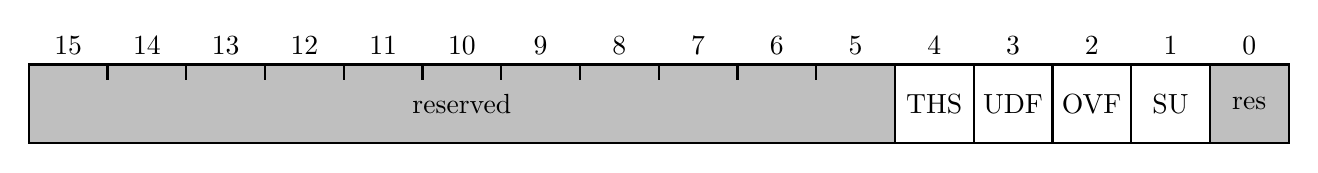
\begin{tikzpicture}
\bitrect{16}{16-\bit}
\robits{0}{11}{reserved}
\rwbits{11}{1}{THS}
\rwbits{12}{1}{UDF}
\rwbits{13}{1}{OVF}
\rwbits{14}{1}{SU}
\robits{15}{1}{res}
\end{tikzpicture}
\end{center}
\begin{itemize}
\item \textbf{THS:} Threshold of modulation FIFO reached. See also section~\ref{mod:fifo}. Reset on its own when the FIFO level drops again.
\item \textbf{UDF:} Modulation FIFO underflow. Last sample will be used for modulation until new data arrives. Reset as a new sample is added to the FIFO.
\item \textbf{OVF:} Modulation FIFO overflow. Oldest sample will be overwritten. Reset by disabling the modulation.
\item \textbf{SU:} Source unlocked
\end{itemize}
\subsection{Writing a register}
Writing a register requires the transfer of two words: First the control word selecting the destination address and a second word containing the new register value:
\begin{center}
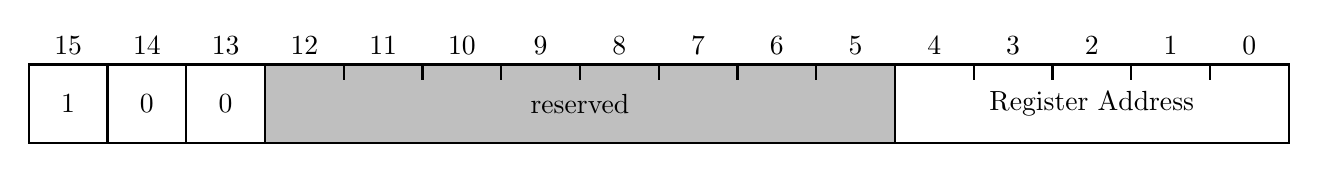
\begin{tikzpicture}
\bitrect{16}{16-\bit}
\rwbits{0}{1}{1}
\rwbits{1}{1}{0}
\rwbits{2}{1}{0}
\robits{3}{8}{reserved}
\rwbits{11}{5}{Register Address}
\end{tikzpicture}
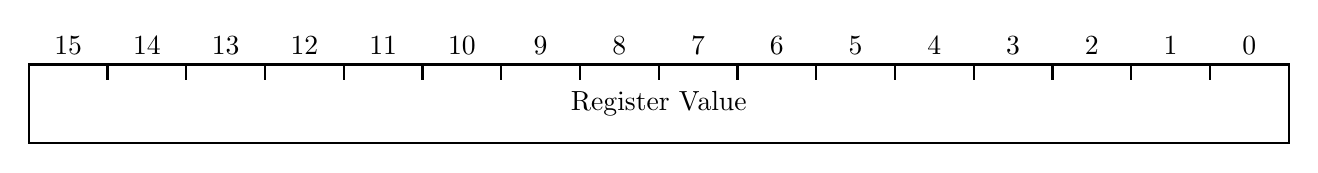
\begin{tikzpicture}
\bitrect{16}{16-\bit}
\rwbits{0}{16}{Register Value}
\end{tikzpicture}
\end{center}
\subsection{Writing the VCO lookup table}
The MAX2871 contains 64 individual VCOs. The correct VCO has to be selected for each frequency. During modulation, the FPGA performs the VCO selection and needs to know the frequency limits for each VCO. It contains a lookup table with a 16-bit entry for each VCO. This table has to be filled before enabling the modulation, as each MAX2871 sample has slightly different VCO limits (see MAX2871 datasheet for algorithm to determine the limits).
Updating a table entry is done by sending two SPI words:
\begin{center}
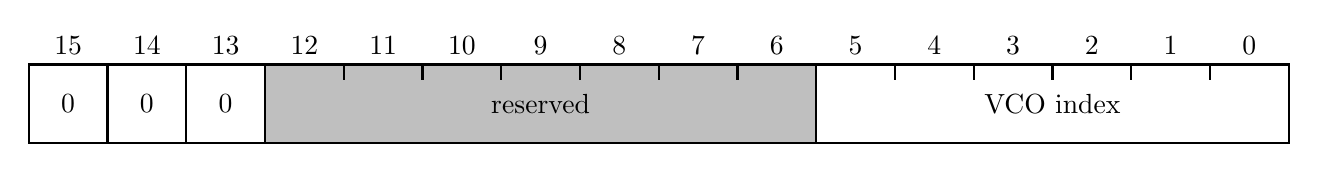
\begin{tikzpicture}
\bitrect{16}{16-\bit}
\rwbits{0}{1}{0}
\rwbits{1}{1}{0}
\rwbits{2}{1}{0}
\robits{3}{7}{reserved}
\rwbits{10}{6}{VCO index}
\end{tikzpicture}
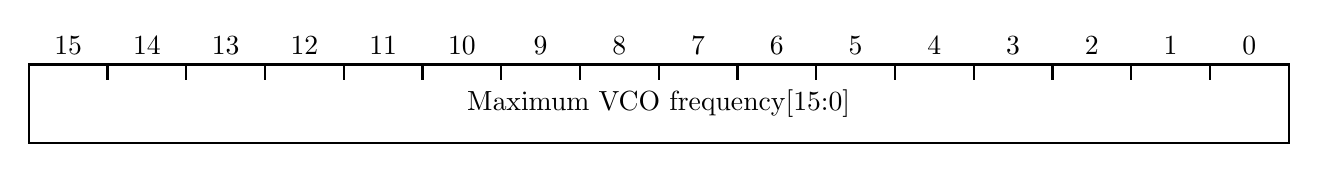
\begin{tikzpicture}
\bitrect{16}{16-\bit}
\rwbits{0}{16}{Maximum VCO frequency[15:0]}
\end{tikzpicture}
\end{center}
The maximum VCO frequency is given in terms of the MAX2871 reference frequency. It is a Q10 fixed point integer.
$$
Maximum VCO frequency[15:0] = \frac{f_{max} * 1024}{f_{reference}}
$$
Example: With a reference frequency $f_{reference} = 104 MHz$ and a maximum usable frequency of the VCO of $f_{max} = 3718 MHz$, set the maximum VCO frequency value to 36608.

\subsection{Modulation FIFO handling}
\label{mod:fifo}
The modulation module contains a data FIFO for the modulation data (samples). Each sample is an 8-bit word that determines the modulation state. The modulation moves on to the next sample at a rate determined by MOD\_PHASE\_INC. The FIFO has a size of 2048 samples. It can only be written to, reading back data from the FIFO is not possible.

The FIFO also has three interrupts (see status register, section~ref{reg:status}):
\begin{itemize}
\item \textbf{Overflow:} Asserted when samples have been written to an already full FIFO. This bit does not clear even if the FIFO level drops afterwards. The modulation has to be disabled to reset this bit. Disabling the modulation also clears the FIFO.
\item \textbf{Underflow:} Asserted when no more samples are available in the FIFO but the modulation module is scheduled to move to the next sample. The modulation will continue to use the last available sample until new data is written to the FIFO. This bit is cleared by writing new FIFO data.
\item \textbf{Threshold crossed:} Asserted when the FIFO contains at least MOD\_FIFO\_THRESHOLD (see section~ref{reg:mod:fifo:thresh}) samples.
\end{itemize}

\subsubsection{Writing to the modulation FIFO}
It is only possible to write to bytes at a time to the modulation FIFO. Initiate the write by sending the command word:
\begin{center}
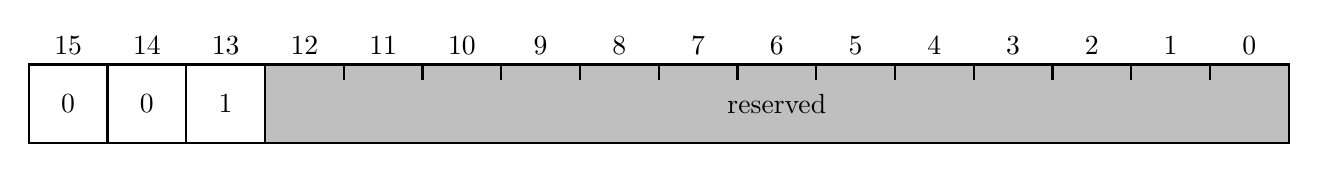
\begin{tikzpicture}
\bitrect{16}{16-\bit}
\rwbits{0}{1}{0}
\rwbits{1}{1}{0}
\rwbits{2}{1}{1}
\robits{3}{13}{reserved}
\end{tikzpicture}
\end{center}
Follow up the same SPI transaction (NSS has to stay low) with as many words as desired, each word containing two FIFO samples:
\begin{center}
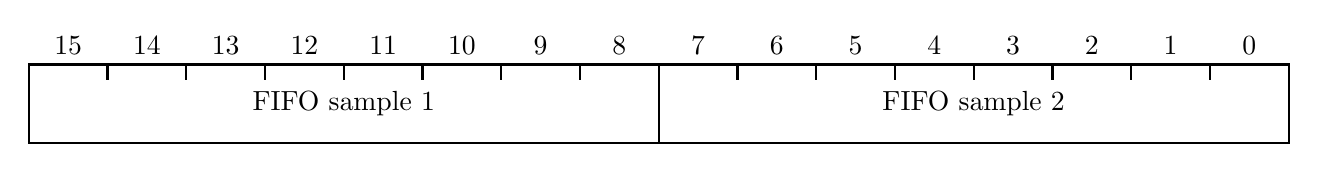
\begin{tikzpicture}
\bitrect{16}{16-\bit}
\rwbits{0}{8}{FIFO sample 1}
\rwbits{8}{8}{FIFO sample 2}
\end{tikzpicture}
\end{center}
FIFO sample 1 is added to the FIFO first, followed by FIFO sample 2.

\section{Registers}
\subsection{Interrupt Mask Register: 0x00}
\begin{center}
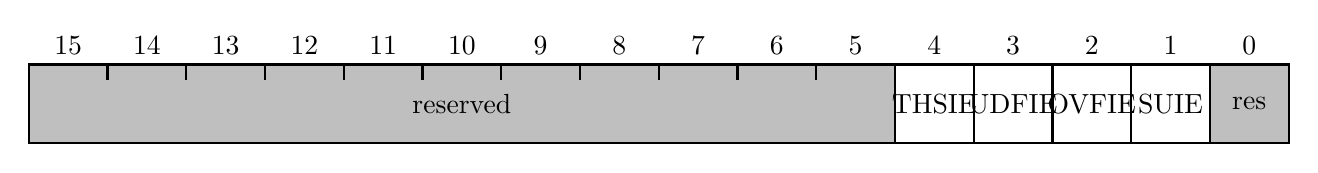
\begin{tikzpicture}
\bitrect{16}{16-\bit}
\robits{0}{11}{reserved}
\rwbits{11}{1}{THSIE}
\rwbits{12}{1}{UDFIE}
\rwbits{13}{1}{OVFIE}
\rwbits{14}{1}{SUIE}
\robits{15}{1}{res}
\end{tikzpicture}
\end{center}
\begin{itemize}
\item \textbf{THSIE:} FIFO threshold crossed interrupt enable
\item \textbf{UDFIE:} FIFO underflow interrupt enable 
\item \textbf{OVFIE:} FIFO overflow interrupt enable
\item \textbf{SUIE:} Source unlocked interrupt enable
\end{itemize}

\subsection{Source Control Register: 0x01}
\begin{center}
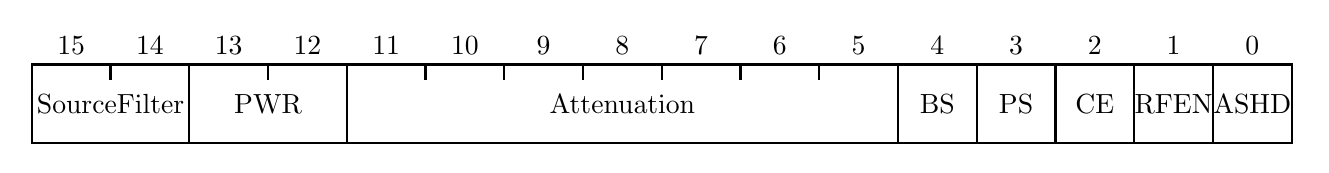
\begin{tikzpicture}
\bitrect{16}{16-\bit}
\rwbits{0}{2}{SourceFilter}
\rwbits{2}{2}{PWR}
\rwbits{4}{7}{Attenuation}
\rwbits{11}{1}{BS}
\rwbits{12}{1}{PS}
\rwbits{13}{1}{CE}
\rwbits{14}{1}{RFEN}
\rwbits{15}{1}{ASHD}
\end{tikzpicture}
\end{center}
\begin{itemize}
\item \textbf{SourceFilter:} Low pass filter selection for source signal
\begin{center}
\begin{tabular}{ c|c }
Setting & Selected Band\\
 \hline
00 & \SIrange{0}{900}{\mega\hertz}\\
01 & \SIrange{900}{1800}{\mega\hertz}\\
10 & \SIrange{1800}{3500}{\mega\hertz}\\
11 & \SIrange{3500}{6000}{\mega\hertz}\\
\end{tabular}
\end{center}
\item \textbf{PWR:} Power setting of source PLL. Will be written to register 4, bits [4:3] of the source PLL, controlling the output power of output A.
\begin{center}
\begin{tabular}{ c|c }
Setting & Selected Power\\
 \hline
00 & \SI{-4}{\dBm}\\
01 & \SI{-1}{\dBm}\\
10 & \SI{2}{\dBm}\\
11 & \SI{5}{\dBm}\\
\end{tabular}
\end{center}
\item \textbf{Attenuator:} Attenuation of source signal in \SI{0.25}{\decibel}.
\item \textbf{BS: Band select.} Set to 0 for highband, set to 1 for lowband.
\item \textbf{PS: Port select.} Set to 0 for Port 1, set to 1 for Port 2.
\item \textbf{CE: Source chip enable.} 
\item \textbf{RFEN: Source RF enable.}
\item \textbf{ASHD: Amplifier disable.}
\end{itemize}

\subsection{Modulation control register: 0x02}
\begin{center}
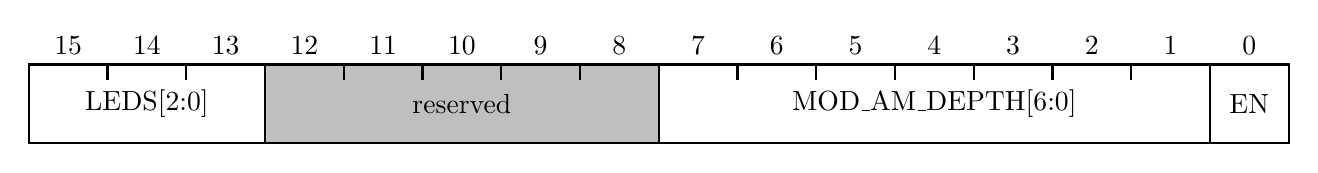
\begin{tikzpicture}
\bitrect{16}{16-\bit}
\rwbits{0}{3}{LEDS[2:0]}
\robits{3}{5}{reserved}
\rwbits{8}{7}{MOD\_AM\_DEPTH[6:0]}
\rwbits{15}{1}{EN}
\end{tikzpicture}
\end{center}
\begin{itemize}
\item \textbf{LEDS:} User LED status:
\begin{center}
\begin{tabular}{ c|c }
LED num & Function\\
 \hline
0 & Debug\\
1 & Ready\\
2 & Ext. reference\\
\end{tabular}
\end{center}
\item \textbf{MOD\_AM\_DEPTH:} Depth of amplitude modulation. Higher values of the modulation sample result in deeper modulation. This setting determines the maximum depth. 127 is equivalent to 100\% modulation.
\item \textbf{EN: Enable modulation.} Set to 1 to enable the modulation. For the modulation to actually start, AUX3 also has to be pulled low. Set to 0 to disable the modulation (when changing settings or to clear the modulation FIFO).
\end{itemize}

\subsection{Modulation phase increment register: 0x03}
\begin{center}
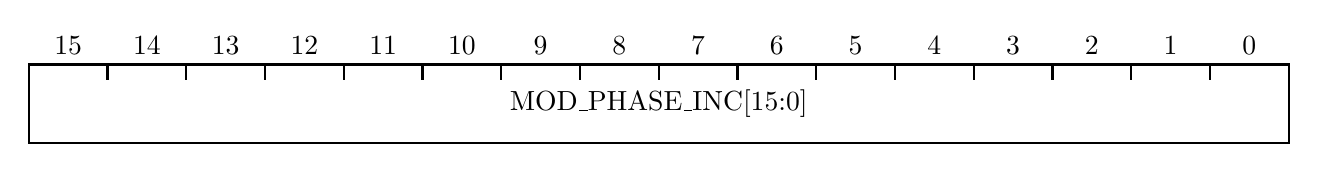
\begin{tikzpicture}
\bitrect{16}{16-\bit}
\rwbits{0}{16}{MOD\_PHASE\_INC[15:0]}
\end{tikzpicture}
\end{center}

Determines the rate at which the modulation module consumes samples:
$$
f_{sample} = \frac{102.4 MHz * MOD\_PHASE\_INC}{2^{27}}
$$
Example: set to 26214 for a sample rate of approximately 20 kHz.

\subsection{Modulation center frequency LSB register: 0x04}
\label{reg:mod:center:lsb}
\begin{center}
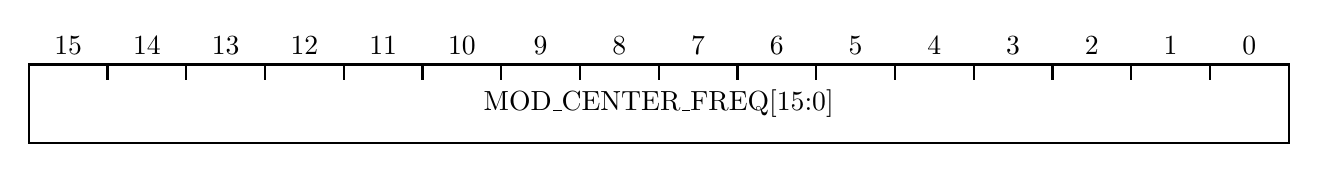
\begin{tikzpicture}
\bitrect{16}{16-\bit}
\rwbits{0}{16}{MOD\_CENTER\_FREQ[15:0]}
\end{tikzpicture}
\end{center}
\begin{itemize}
\item \textbf{MOD\_CENTER\_FREQ[32:0]:} See also other registers for remaining bits (sections~\ref{reg:mod:center:msb} and \ref{reg:mod:dev:msb}). Sets the center frequency of the frequency modulation. It is given in terms of the MAX2871 reference frequency. It is a Q27 fixed point integer.
$$
MOD\_CENTER\_FREQ[32:0] = \frac{f_{center} * 2^{27}}{f_{reference}}
$$
\end{itemize}

\subsection{Modulation center frequency MSB register: 0x05}
\label{reg:mod:center:msb}
\begin{center}
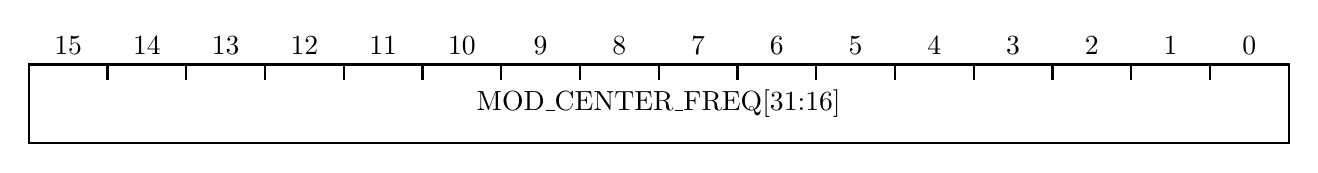
\begin{tikzpicture}
\bitrect{16}{16-\bit}
\rwbits{0}{16}{MOD\_CENTER\_FREQ[31:16]}
\end{tikzpicture}
\end{center}

\subsection{Modulation deviation frequency LSB register: 0x06}
\label{reg:mod:dev:lsb}
\begin{center}
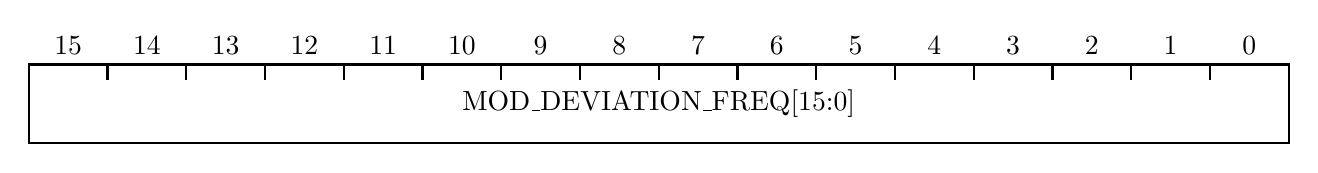
\begin{tikzpicture}
\bitrect{16}{16-\bit}
\rwbits{0}{16}{MOD\_DEVIATION\_FREQ[15:0]}
\end{tikzpicture}
\end{center}

\begin{itemize}
\item \textbf{MOD\_DEVIATION\_FREQ[25:0]:} See also other register for remaining bits (section~\ref{reg:mod:dev:msb}). Sets the maximum deviation from the center frequency during frequency modulation. It is given in terms of the MAX2871 reference frequency. It is a Q27 fixed point integer. As it only has 26 bits, the maximum deviation is half the reference frequency.
$$
MOD\_DEVIATION\_FREQ[25:0] = \frac{f_{max_deviation} * 2^{27}}{f_{reference}}
$$
\end{itemize}

\subsection{Modulation deviation frequency MSB register: 0x07}
\label{reg:mod:dev:msb}
\begin{center}
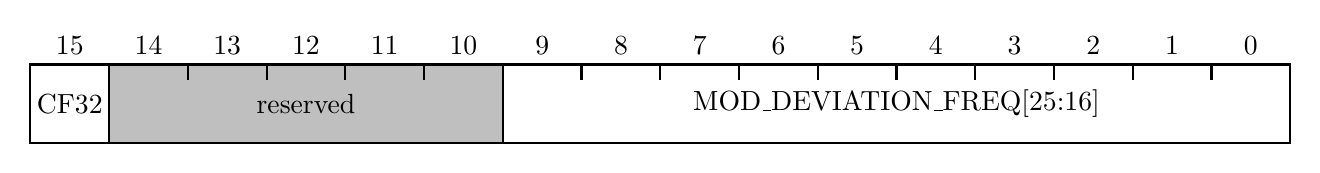
\begin{tikzpicture}
\bitrect{16}{16-\bit}
\rwbits{0}{1}{CF32}
\robits{1}{5}{reserved}
\rwbits{6}{10}{MOD\_DEVIATION\_FREQ[25:16]}
\end{tikzpicture}
\end{center}
\begin{itemize}
\item \textbf{CF32:} Most significant bit of MOD\_CENTER\_FREQ.
\end{itemize}

\subsection{Minimum VCO frequency LSB register: 0x08}
\label{reg:mod:minvco:lsb}
\begin{center}
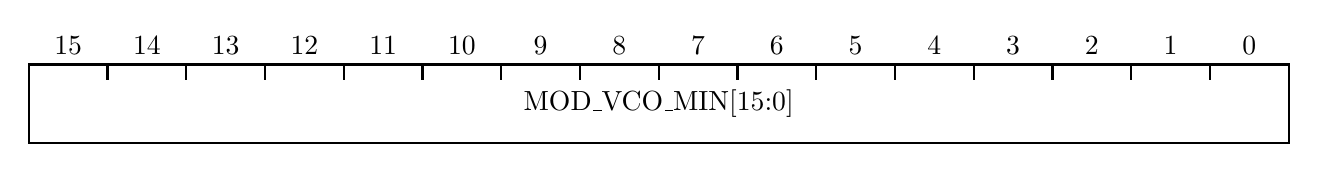
\begin{tikzpicture}
\bitrect{16}{16-\bit}
\rwbits{0}{16}{MOD\_VCO\_MIN[15:0]}
\end{tikzpicture}
\end{center}
\begin{itemize}
\item \textbf{MOD\_VCO\_MIN[31:0]:} See also other register for remaining bits (section~\ref{reg:mod:minvco:msb}). Sets the minimal allowed undivided VCO frequency. Used to determine the VCO divider when changing frequencies. It is given in terms of the MAX2871 reference frequency. It is a Q27 fixed point integer. Always set this for a minimal undivided VCO frequency of 3 GHz.
$$
MOD\_VCO\_MIN[31:0] = \frac{f_{min_vco} * 2^{27}}{f_{reference}}
$$
\end{itemize}
For the default reference frequency of 104 MHz, set this value to 3871665231.

\subsection{Minimum VCO frequency MSB register: 0x05}
\label{reg:mod:minvco:msb}
\begin{center}
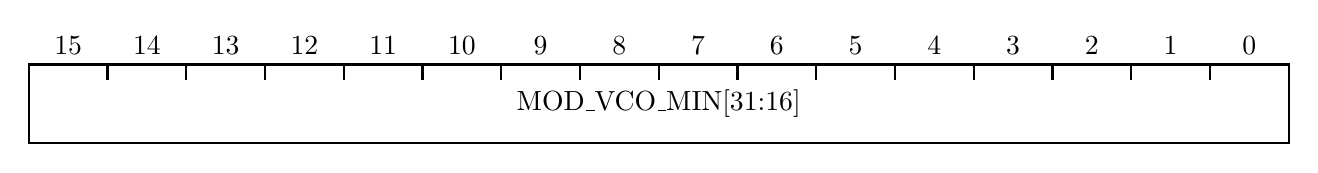
\begin{tikzpicture}
\bitrect{16}{16-\bit}
\rwbits{0}{16}{MOD\_VCO\_MIN[31:16]}
\end{tikzpicture}
\end{center}

\subsection{Modulation FIFO threshold register: 0x0A}
\label{reg:mod:fifo:thresh}
\begin{center}
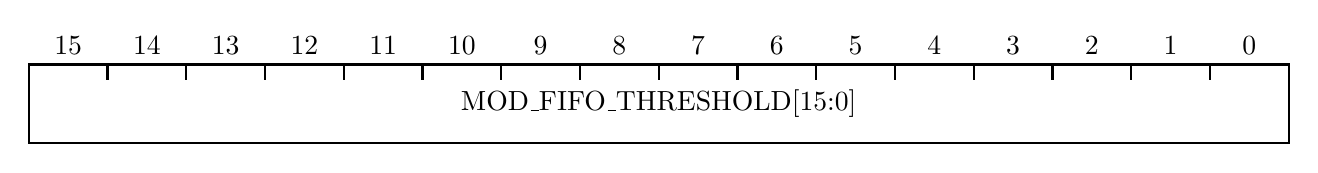
\begin{tikzpicture}
\bitrect{16}{16-\bit}
\rwbits{0}{16}{MOD\_FIFO\_THRESHOLD[15:0]}
\end{tikzpicture}
\end{center}
\begin{itemize}
\item \textbf{MOD\_FIFO\_THRESHOLD[15:0]:} Number of samples in the FIFO after which the FIFO threshold interrupt is asserted.
\end{itemize}

\end{document}